\chapter{Arduino IDE 2.3.2}
\section{Overview of Arduino IDE}

It is an open source official Arduino software which used for editing, uploading and compiling codes in to the Arduino module. It is a cross-platform software which is available for Operating Systems like Windows, Linux, macOS. It runs on Java platform and supports a range of Arduino modules. It supports C and C++ languages. The microcontrollers present on the Arduino boards are programmed which accepts the information in the form of code. The program written in the IDE is called a sketch which will generate a Hex file which is then transferred and uploaded in the controller. The IDE environment is made up of two parts: an editor and a compiler. The editor is used to write the required code, while the compiler is used to compile and upload the code to the Arduino Module. The Menu bar has options such as File in which there are many options including Opening a new file or existing, Examples-in which we can find sketches for different applications like Blink, Fade etc. There is an error console at the bottom of the screen for displaying errors. The Arduino IDE features a new sidebar, making the most commonly used toolsas. ~\ref{ide-2-overview} \cite{arduinodescription:2024} \cite{arduino_ide_environment:2025}


\begin{itemize}
	\item \textbf{Verify / Upload}- compile and upload your code to your Arduino Board.
	\item \textbf{Select Board and Port}- detected Arduino boards automatically show up here, along with the port number.
	\item \textbf{Sketchbook}- here you will find all of your sketches locally stored on your computer. Additionally, you can sync with the Arduino Cloud, and also obtain your sketches from the online environment.
	\item \textbf{Boards Manager}- browse through Arduino and third party packages that can be installed. For example, using a MKR WiFi 1010 board requires the Arduino SAMD Boards package installed.
	\item \textbf{Library Manager}- browse through thousands of Arduino libraries, made by Arduino and its community.
	\item \textbf{Debugger}- test and debug programs in real time.
	\item \textbf{Search}- search for keywords in your code.
	\item \textbf{Open Serial Monitor}- opens the Serial Monitor tool, as a new tab in the console.
\end{itemize}

\begin{figure}
	\begin{center}
		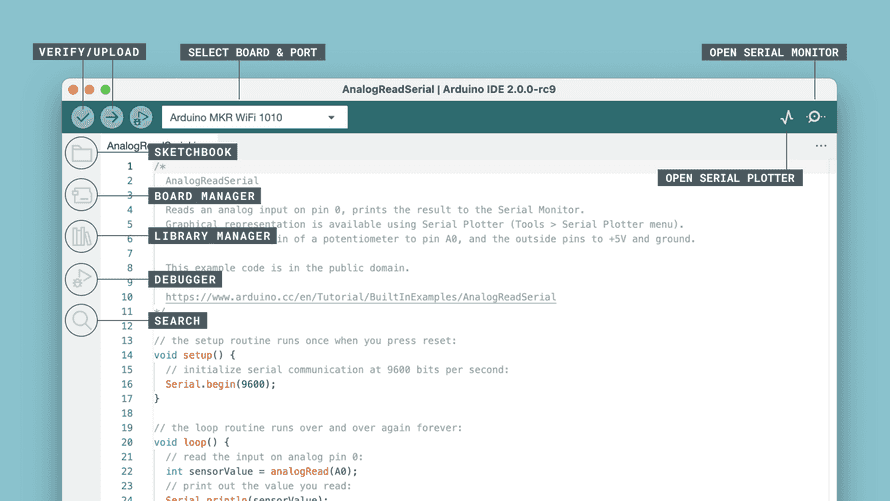
\includegraphics[width=0.7\linewidth]{Images/Arduino/ide-2-overview.png}
		\caption{Overview}
		\label{ide-2-overview}
	\end{center}
\end{figure}

\section{Installation on MacOS}

To install the Arduino IDE, we need to download the latest version from the Arduino webpage \url{https://www.arduino.cc/en/software}. We can select the version based on the operating system we are using. Here we are installing Arduino 2.3.2 for a MacOS(Sonoma 14.4.1) operating system. The set up file name is \FILE{arduino-ide\_2.3.2\_macOS\_64bit.dmg} and the size of it is 1,93,600 KB. The file is in Zip format. If you use Safari it will be automatically extracted. If you use a different browser you may need to extract it manually. The most recent offline arduino IDE 2.3.2 can be seen in Figure ~\ref{fig:ArduinoIDE Create Agent Installation} it is also supportive for all operating systems \cite{arduino_ide_mac_tutorial:2025}.

\begin{center}
	
	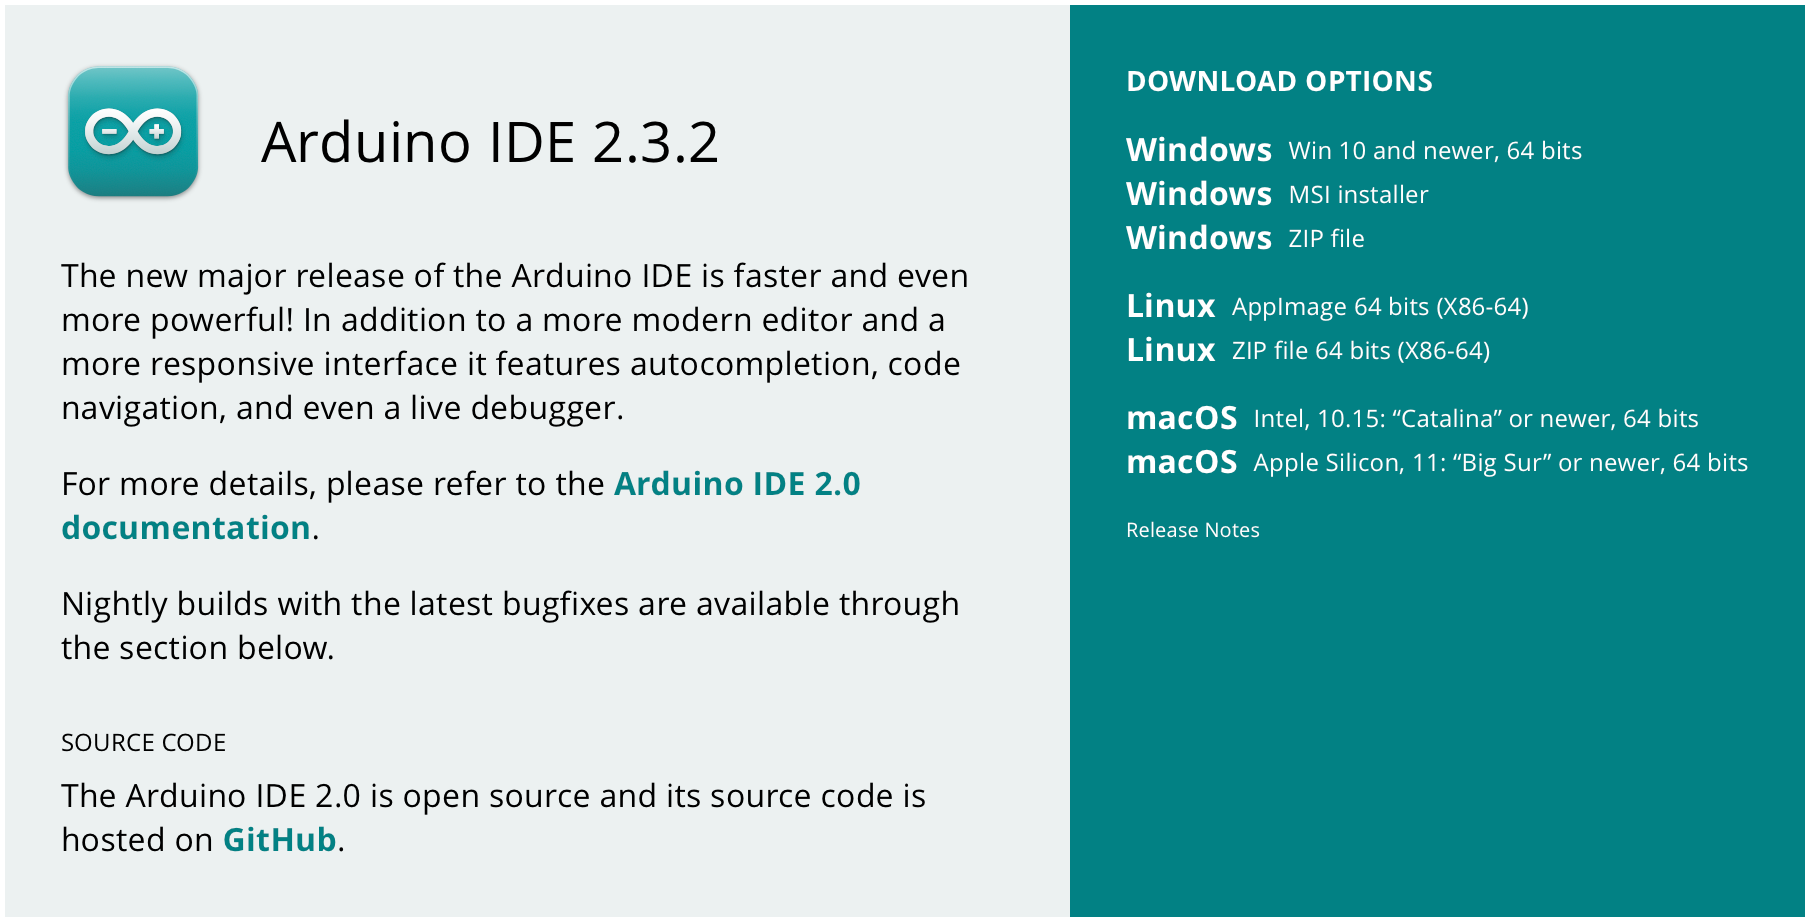
\includegraphics[width=0.7\linewidth]{images/ArduinoIDE/ArduinoIdeCreateAgentInstallation.png}
	%\label{fig:ArduinoIDE Create Agent Installation}
	\captionof{figure}{ArduinoIDE Create Agent Installation}
	\label{fig:ArduinoIDE Create Agent Installation}
\end{center}

\begin{center}
	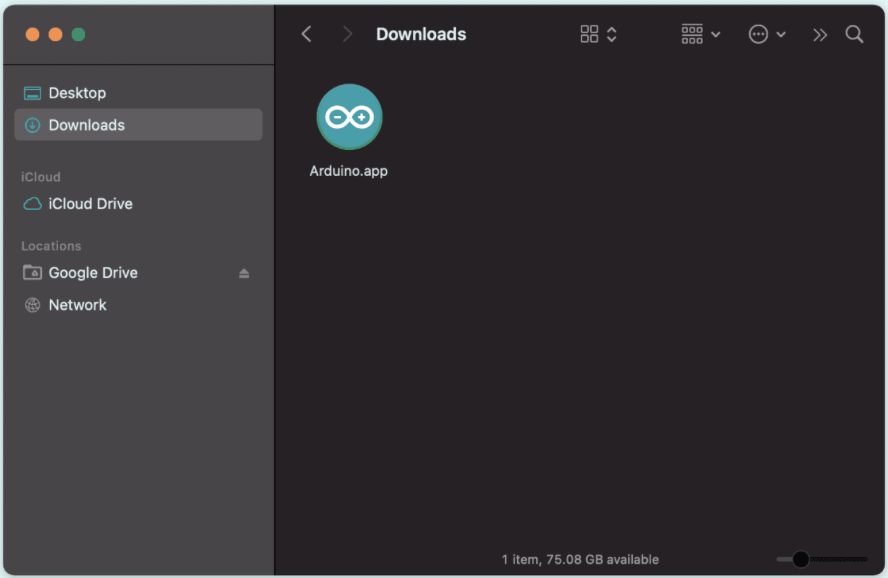
\includegraphics[width=0.7\linewidth]{images/ArduinoIDE/OpenTheDownloadFolder.png}
	\captionof{figure}{Open the Downloadf folder}
\end{center}

Copy the Arduino application bundle into the Applications folder (or elsewhere on your computer) then it look like Figure ~\ref{CopyApplicationFolder}

\begin{figure}
\begin{center}
	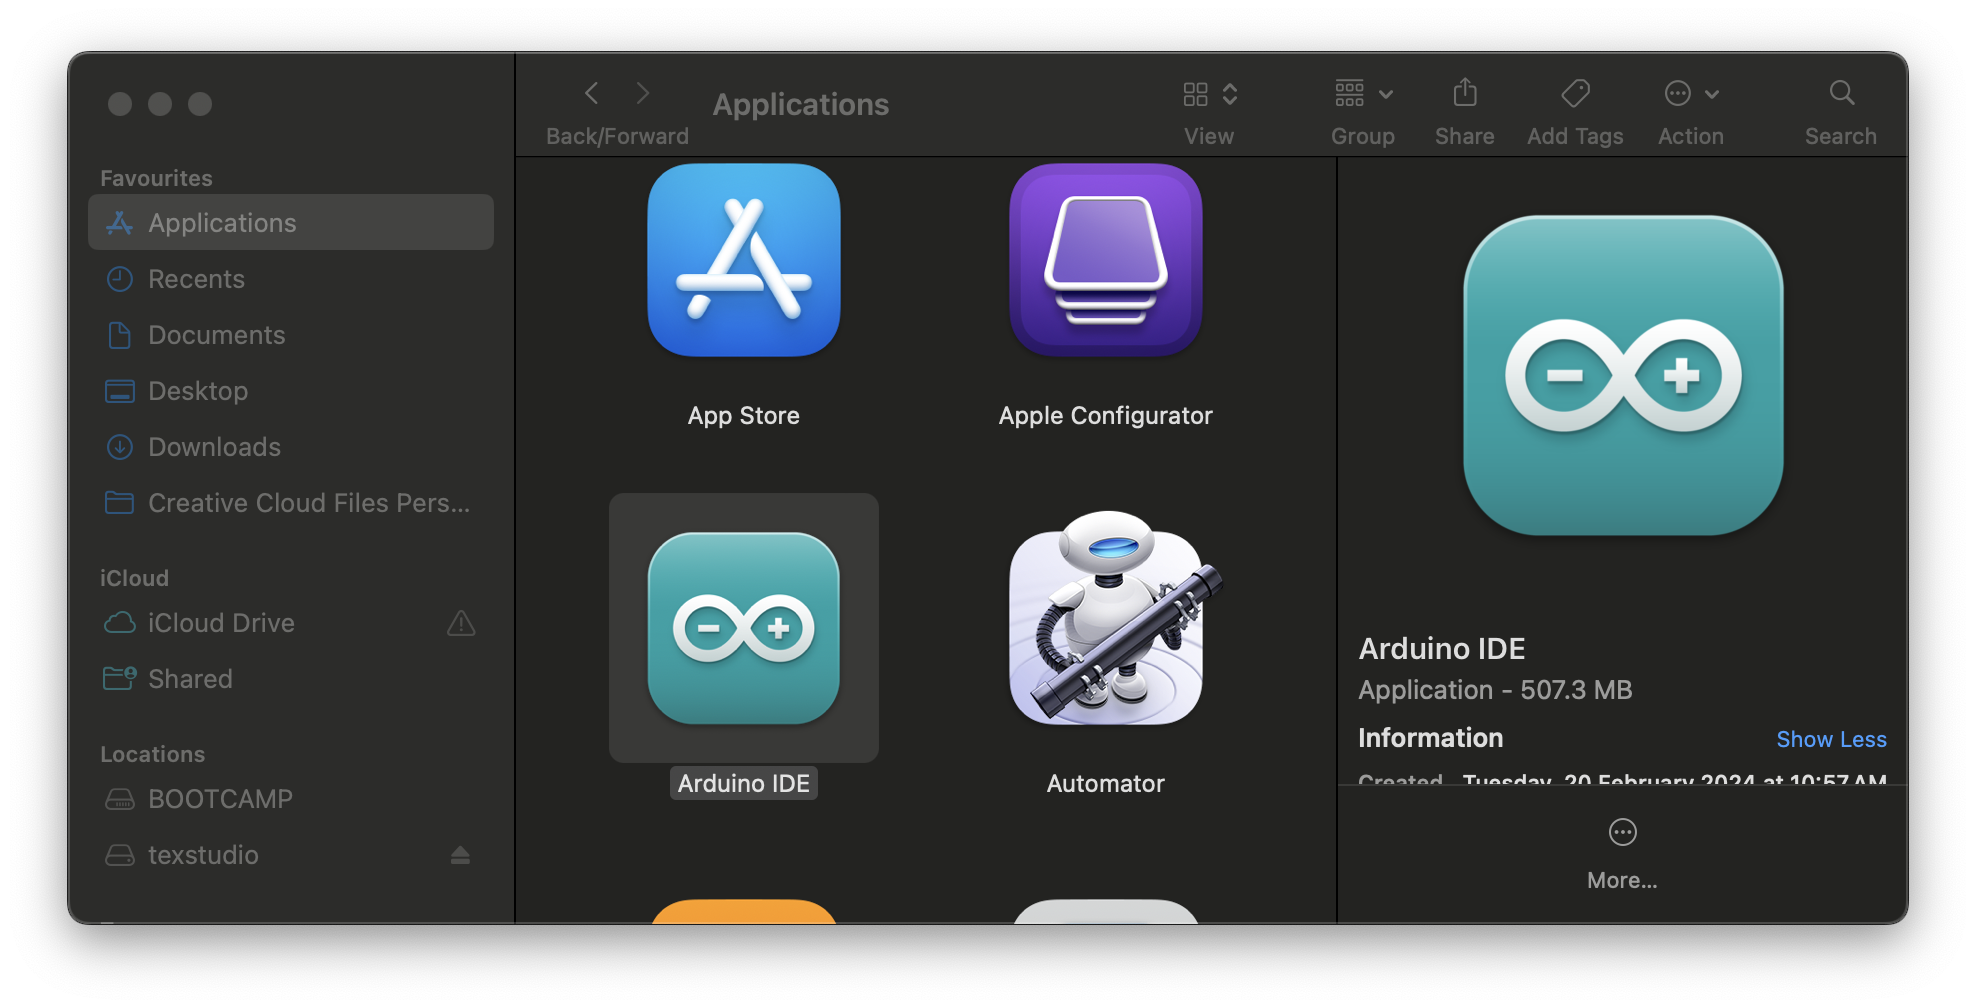
\includegraphics[width=0.7\linewidth]{images/ArduinoIDE/CopyToTheApplicationsFolder.png}
	\captionof{figure}{Copy to the Applications folder}
	\label{CopyApplicationFolder}
\end{center}
\end{figure}

It can be seen from the Figure \ref{fig:Arduino Sketch} that the basic Arduino sketch has two parts. 

\begin{itemize}
	\item \SHELL{void setup():} This function returns void and we do the intiliaztion such as the output LED color, specifying the core etc
	\item \SHELL{void loop():} In this function we define functions which are to be performed throughout the loop. These codes are placed between paranthesis {} and each function has a return type, here it has void return type.
\end{itemize}

\begin{center}
	\label{fig:Arduino Sketch}
	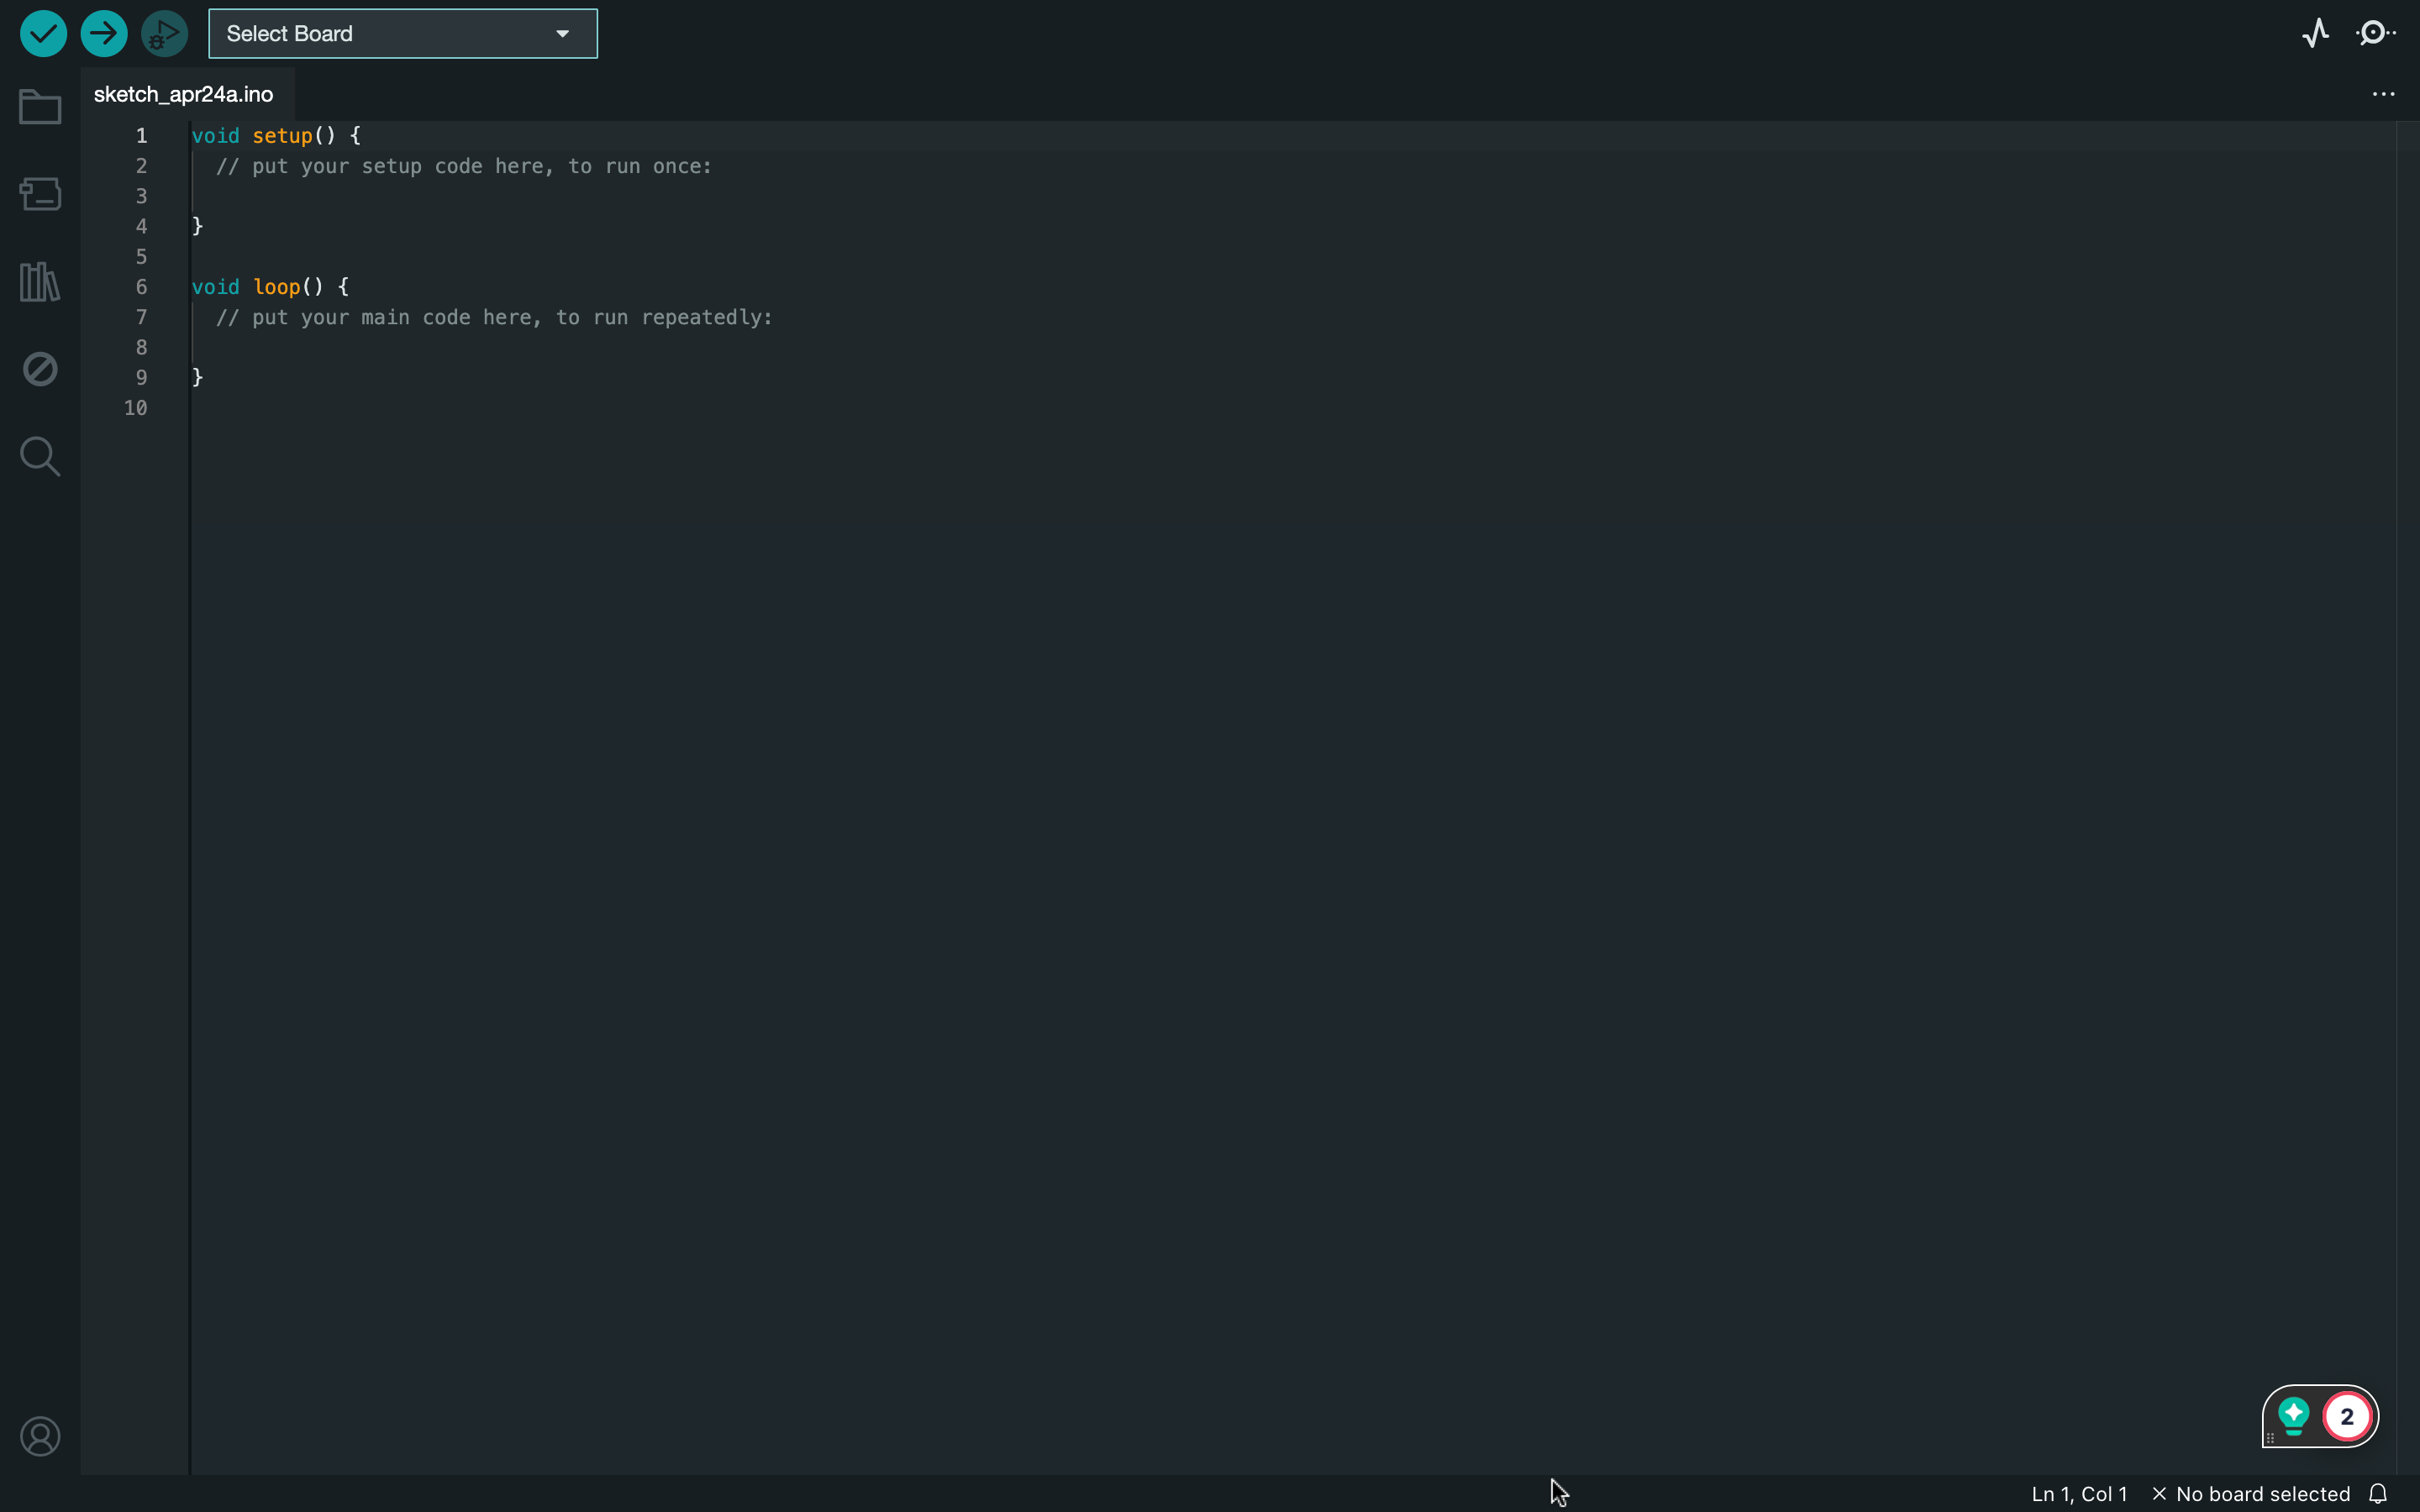
\includegraphics[width=0.7\linewidth]{images/ArduinoIDE/ArduinoIDESketch.png}
	\captionof{figure}{Arduino Sketch}
\end{center}

	
\section{Installation on Windows}
	
	\subsection{Download}
		You can easily download the editor from the Arduino Software page.~\ref{Download} \cite{arduino_ide_windows_tutorial:2025}
		
		\begin{figure}
			\begin{center}
				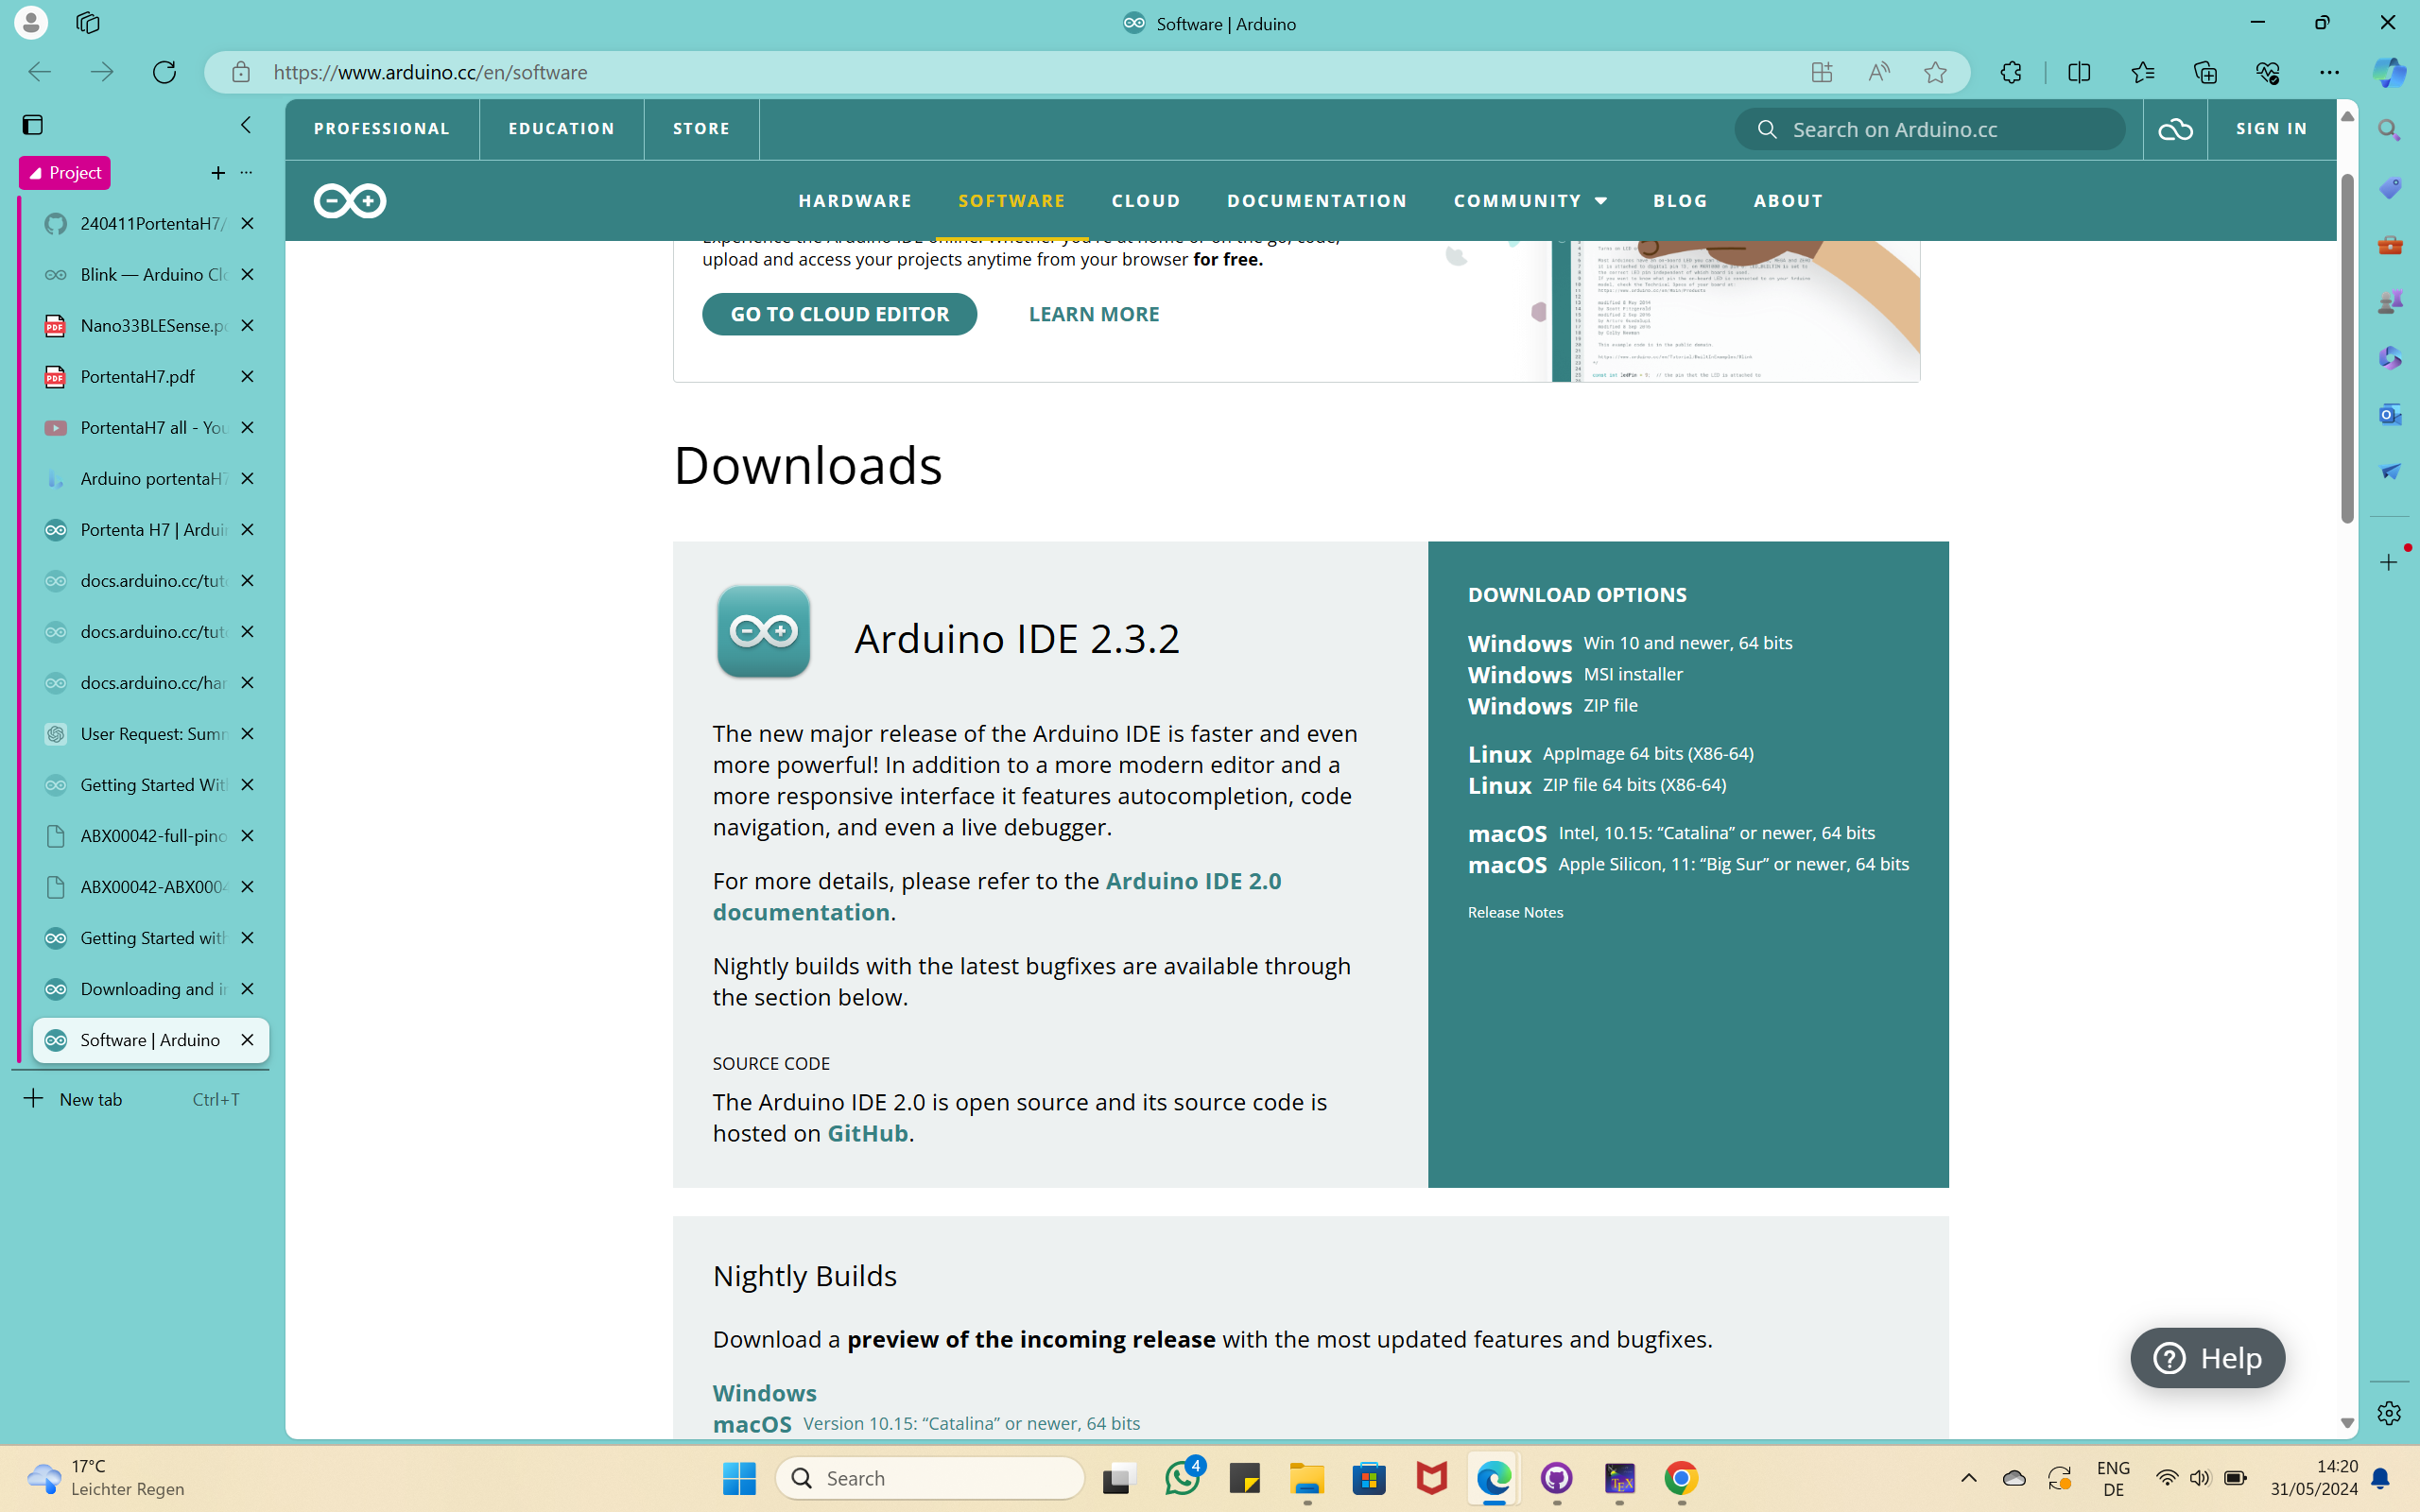
\includegraphics[width=0.7\linewidth]{Images/Arduino/DownloadArduinofile.png}
				\caption{Arduino File}
				\label{Download}
			\end{center}
		\end{figure}
	
	\subsection{Installation}
		To install the Arduino IDE 2 on a Windows computer, simply run the file downloaded from the software page.~\ref{downloading-and-installing-img01} ~\ref{downloading-and-installing-img02} \cite{arduino_ide_windows_tutorial:2025}
		\begin{figure}
			\begin{center}
				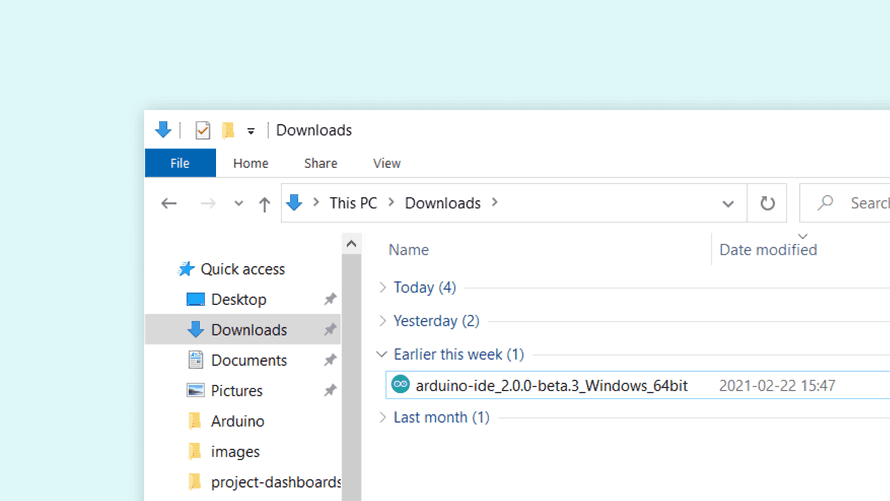
\includegraphics[width=0.7\linewidth]{Images/Arduino/downloading-and-installing-img01.png}
				\caption{Running the installation file}
				\label{downloading-and-installing-img01}
			\end{center}
		\end{figure}
		
		
		\begin{figure}
			\begin{center}
				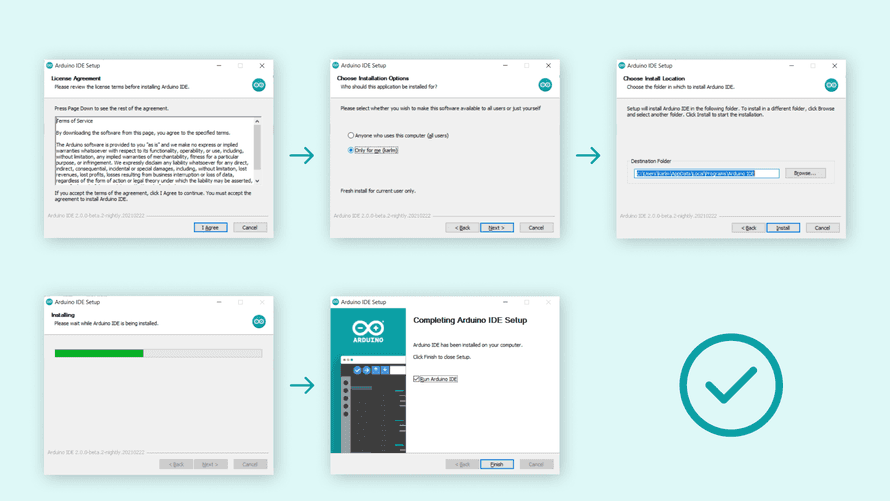
\includegraphics[width=0.7\linewidth]{Images/Arduino/downloading-and-installing-img02.png}
				\caption{Steps for Installation}
				\label{downloading-and-installing-img02}
			\end{center}
		\end{figure}
	
	
\section{Features}
The Arduino IDE 2 is a versatile editor with many features. You can install libraries directly, sync your sketches with Arduino Cloud, debug your sketches and much more. In this section, some of the core features are listed, along with a link to a more detailed article. \cite{arduinodescription:2024} \cite{arduino_ide_environment:2025}

	\subsection{Sketchbook}
		Your sketchbook is where your code files are stored. Arduino sketches are saved as .ino files, and must be stored in a folder of the exact name. For example, a sketch named my sketch.ino must be stored in a folder named my sketch. ~\ref{local-sketchbook}
		
		Typically, your sketches are saved in a folder named Arduino in your Documents folder.
		
		To access your sketchbook, click on the folder icon located in the sidebar.
		\begin{figure}
			\begin{center}
				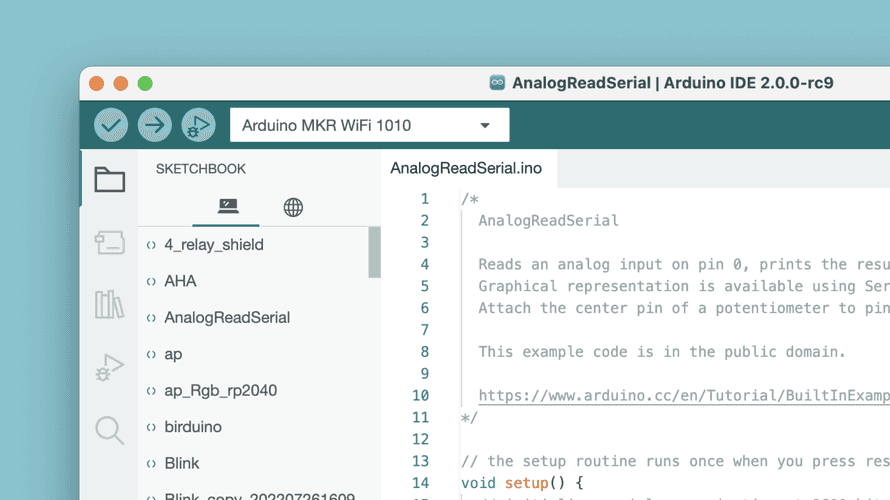
\includegraphics[width=0.7\linewidth]{Images/Arduino/local-sketchbook.png}
				\caption{Sketchbook}
				\label{local-sketchbook}
			\end{center}
		\end{figure}
		
	\subsection{Boards Manager}
	With the Boards Manager, you can browse and install board packages. A board package contains the "instructions" for compiling your code to the boards that are included in the board package. ~\ref{board-manager}
	
	There are several Arduino board packages available, such as avr, samd, megaavr and more.
	\begin{figure}
		\begin{center}
			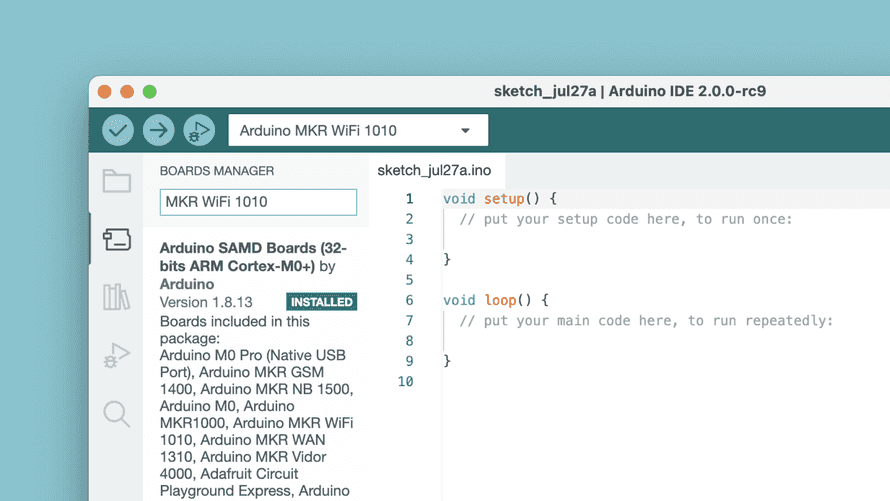
\includegraphics[width=0.7\linewidth]{Images/Arduino/board-manager.png}
			\caption{Board-Manager}
			\label{board-manager}
		\end{center}
	\end{figure}
	
	\subsection{Library Manager}
	With the library manager you can browse and install thousands of libraries. Libraries are extensions of the Arduino API, and makes it easier to for example control a servo motor, read specific sensors, or use a Wi-Fi module. ~\ref{library-manager}
	
	\begin{figure}
		\begin{center}
			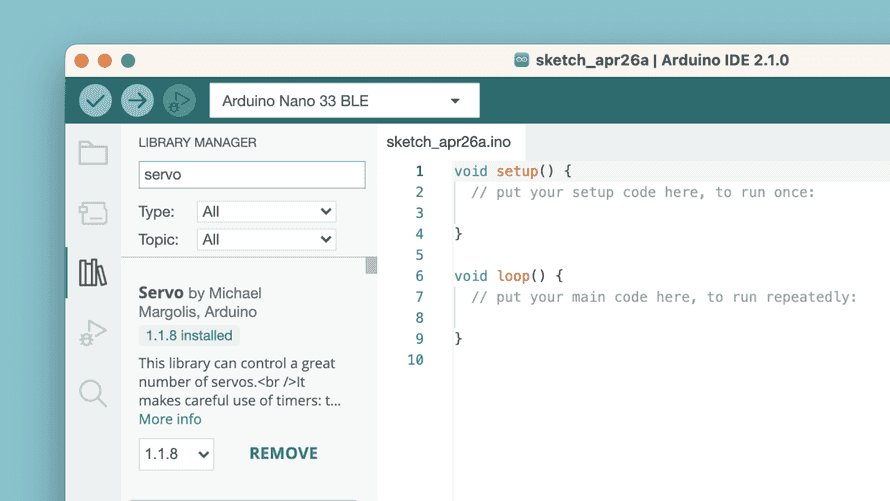
\includegraphics[width=0.7\linewidth]{Images/Arduino/library-manager.png}
			\caption{library-manager}
			\label{library-manager}
		\end{center}
	\end{figure}
	
	\subsection{Serial Monitor}
	The Serial Monitor is a tool that allows you to view data streaming from your board, via for example the Serial.print() command.
	
	Historically, this tool has been located in a separate window, but is now integrated with the editor. This makes it easy to have multiple instances running at the same time on your computer. ~\ref{serial-monitor}
	
	\begin{figure}
		\begin{center}
			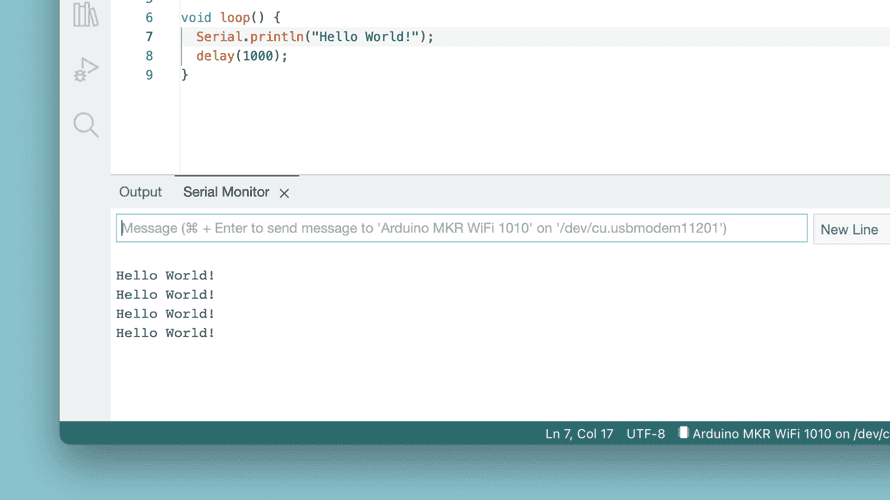
\includegraphics[width=0.7\linewidth]{Images/Arduino/serial-monitor.png}
			\caption{serial-monitor}
			\label{serial-monitor}
		\end{center}
	\end{figure}
	
	\subsection{Serial Plotter}
	The Serial Plotter tool is great for visualizing data using graphs, and to monitor for example peaks in voltage.
	
	You can monitor several variables simultaneously, with options to enable only certain types. 
	
	\subsection{Debugging}
	The debugger tool is used to test and debug programs, hence the name. It can be used to navigate through a program's execution in a controlled manner. ~\ref{Debug}
	
	\begin{figure}
		\begin{center}
			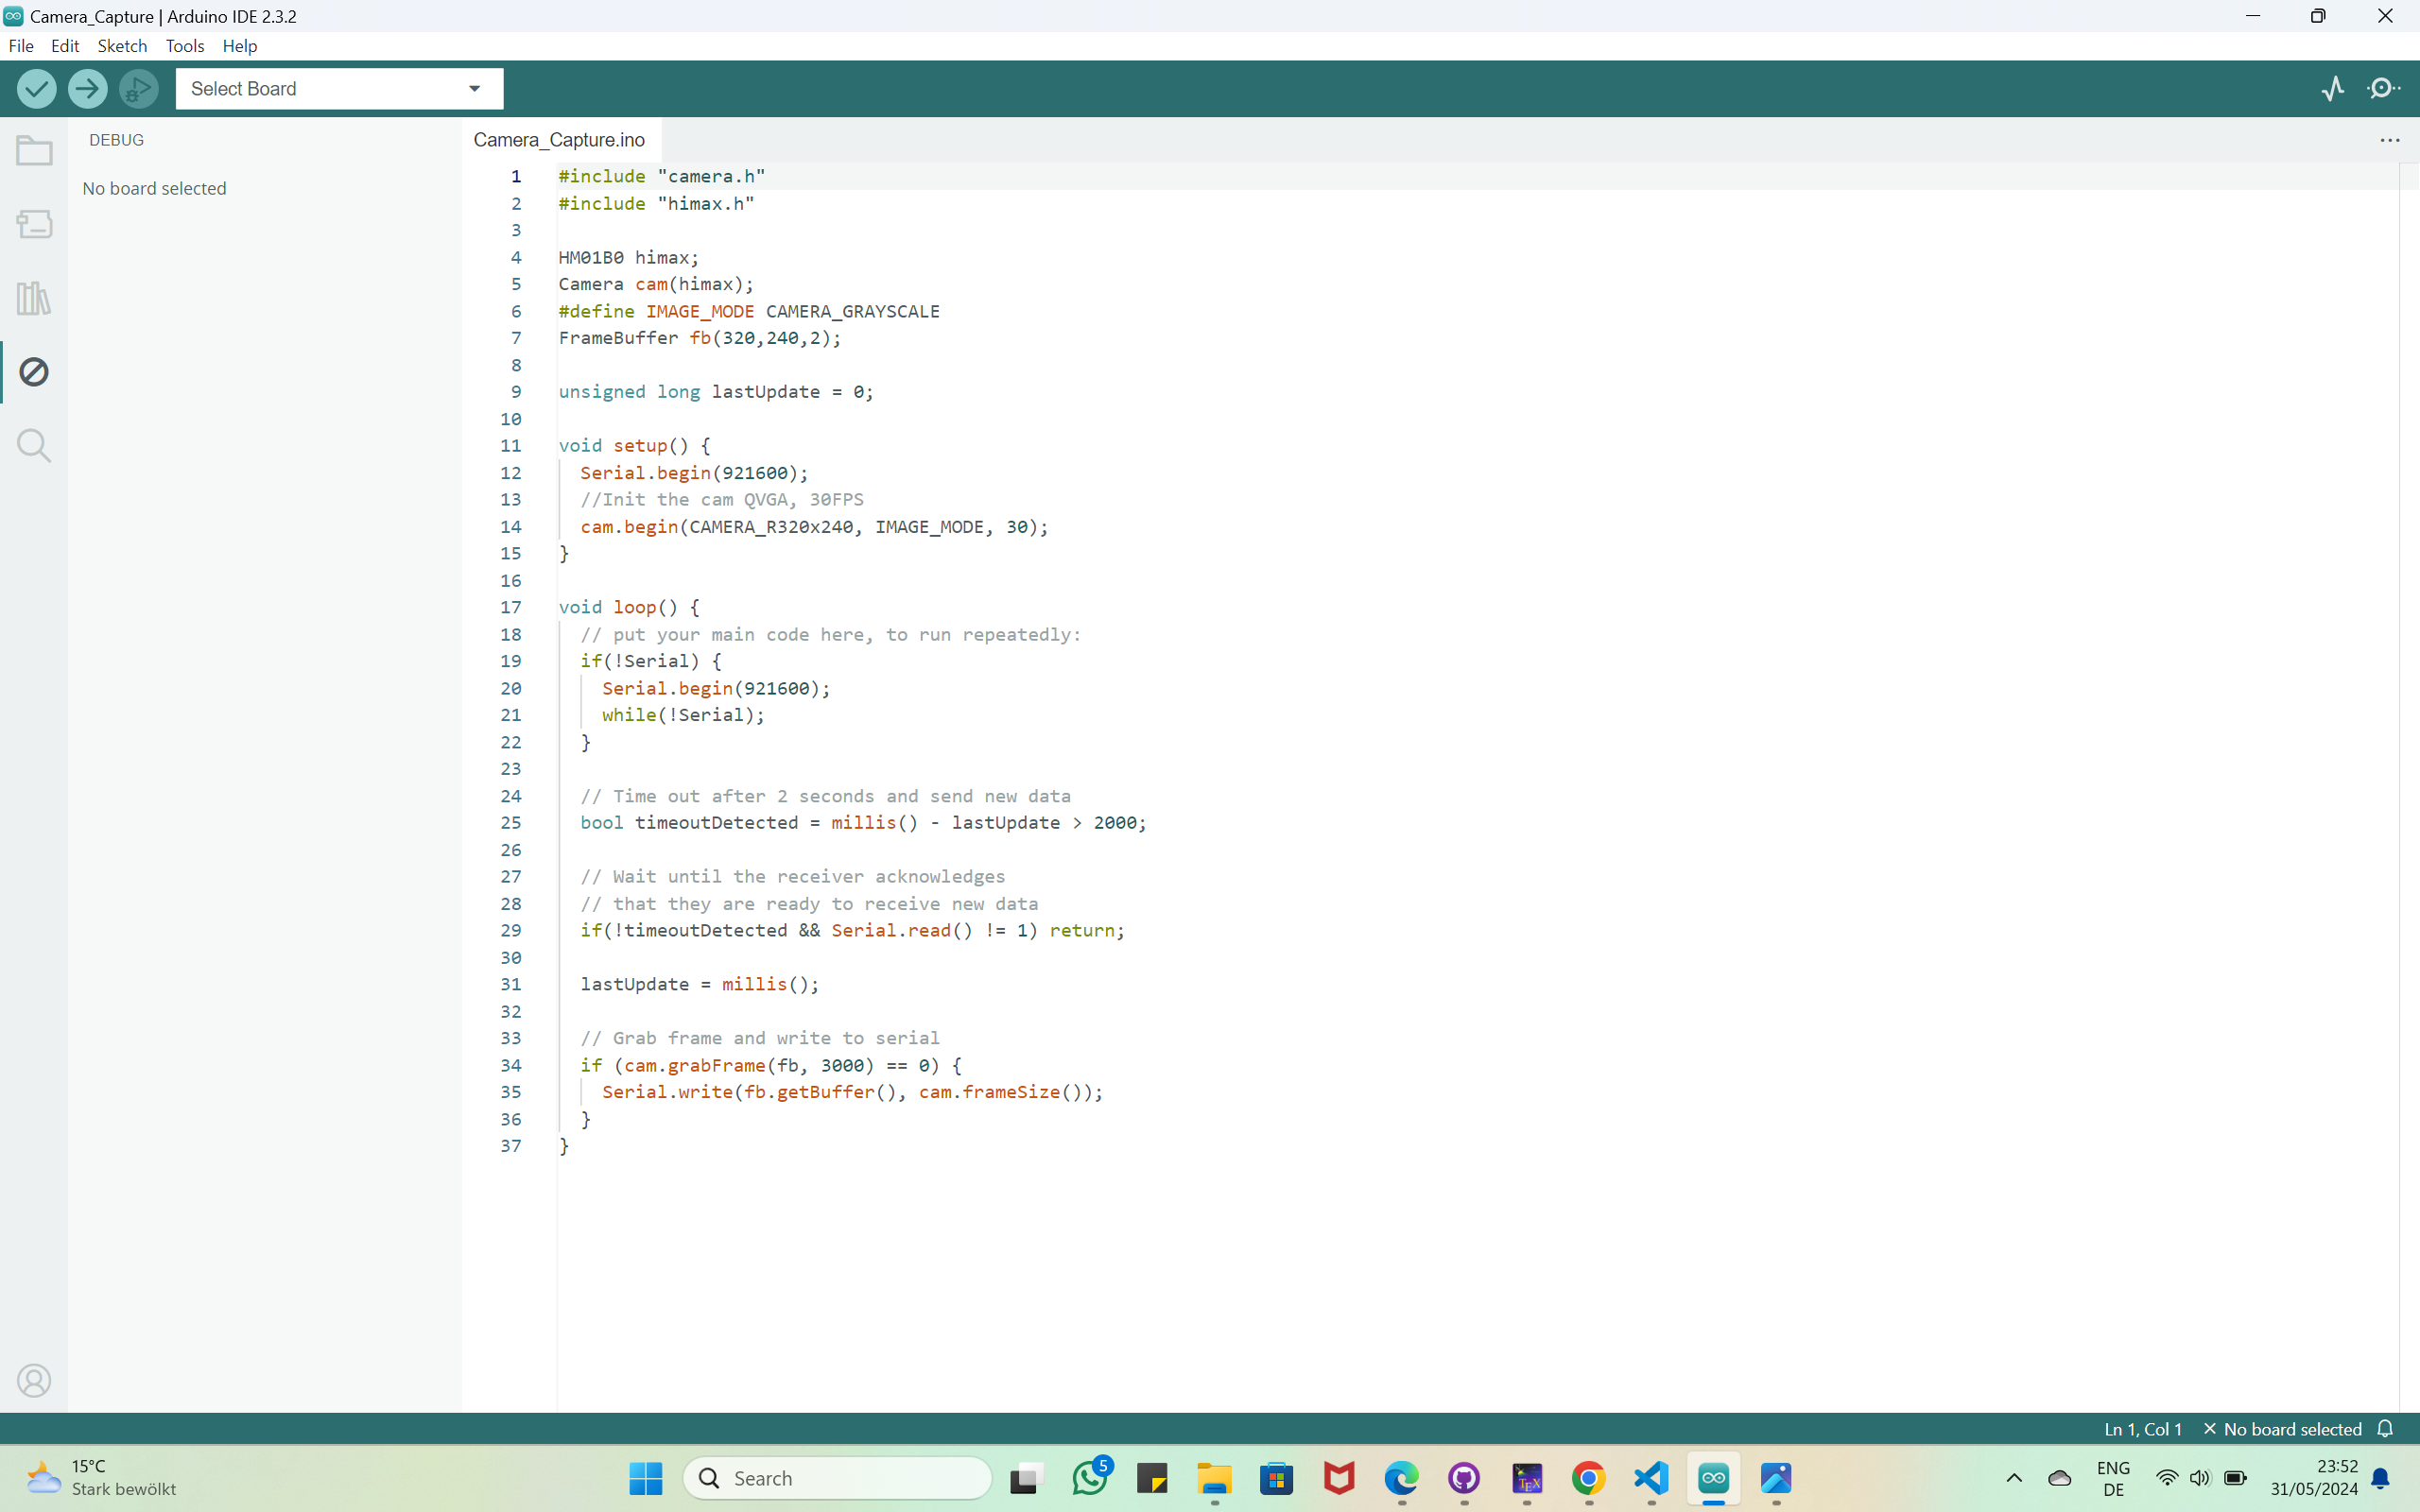
\includegraphics[width=0.7\linewidth]{Images/Arduino/Debug.png}
			\caption{Debugging}
			\label{Debug}
		\end{center}
	\end{figure}
	
	\subsection{Autocompletion}
	Autocompletion is a must-have for code editors, and the 2 version comes well equipped. When writing code, this is useful to understand more about the elements of the Arduino API.
	
	Note that you always need to select your board for autocompletion to work. ~\ref{autocomplete}
	
	\begin{figure}
		\begin{center}
			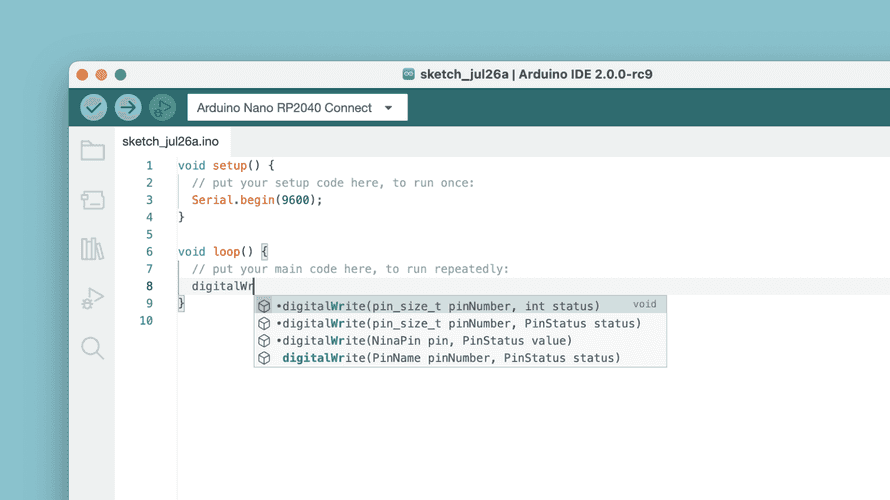
\includegraphics[width=0.6\linewidth]{Images/Arduino/autocomplete.png}
			\caption{autocomplete}
			\label{autocomplete}
		\end{center}
	\end{figure}
	
	
\section{Examples}
An important part of the Arduino Documentation are the example sketches that come bundled with libraries. They will show examples of the functions used in practice, illustrating the intended use and features of a library.

Libraries that come bundled as a part of a boards package may also include libraries, and those libraries often include example sketches.

To open the example sketches bundled in either the libraries you have installed manually or that come bundled in board packages, navigate to \SHELL{File > Examples} and find the library you're searching for in the list that appears. ~\ref{examplesketches}

	\begin{figure}
		\begin{center}
			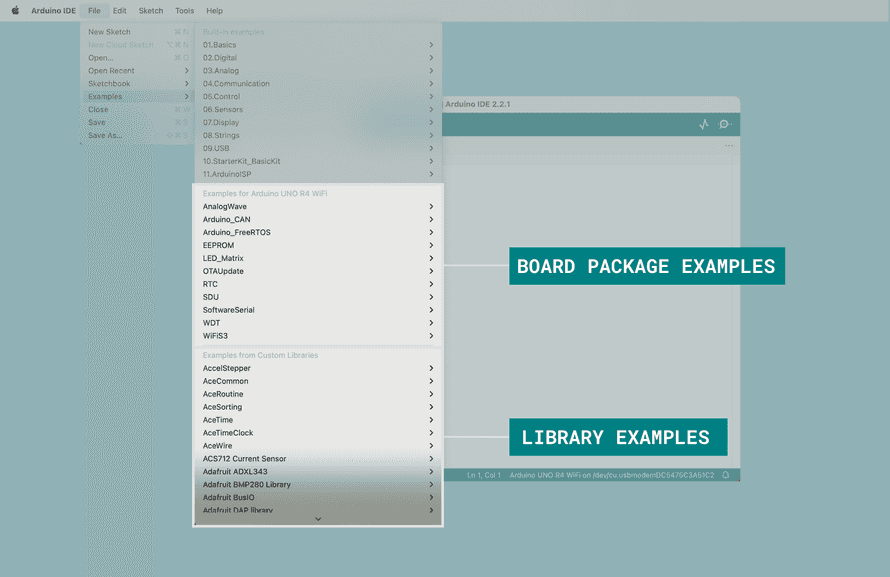
\includegraphics[width=0.7\linewidth]{Images/Arduino/examplesketches.png}
			\caption{Example}
			\label{examplesketches}
		\end{center}
	\end{figure}
	
In the image above, you can see what the examples list looks like when Arduino board is connected to your computer.

From here, you can for example navigate to \SHELL{File > Examples > LED Matrix > MatrixIntro|}and upload the sketch to your board to show the Tetris animation that came pre-loaded on your UNO R4 WiFi when you first took it out of its box.
	

\section{Conclusion}
In this guide, we have presented a series of features and more detailed articles to follow, so that you can enjoy each and every one of the features included in the IDE 2.

